\documentclass[a4paper, 10pt]{article}
\usepackage[utf8x]{inputenc}
\usepackage[norsk]{babel}
\usepackage{natbib}
\usepackage{graphicx}
\usepackage[T1]{fontenc}
\usepackage{amsmath}
\usepackage{mathtools}
\usepackage{hyperref}
\usepackage{listings}

\begin{document}
\begin{titlepage}
\begin{center} 

\vspace*{3cm}
\textsc{\Huge PU5}\\[0.7cm]
\textsc{\medium TTM4100 - Communication Services and Networks}\\[0.3cm]
\textsc{\medium TDT4140 - Software Enigneering}\\[0.3cm]
\textsc{\medium TDT4145 - Data Modeling, Databases and Database Management Systems}\\[0.3cm]
\textsc{\medium TDT4180 - Human-Computer Interaction}\\[0.3cm]

\textbf{\Large Gruppe 6:} \\[0.2cm]
\text{\Large Espen Albert, Finn Inderhaug, Kristoffer Andreas Dalby} \\
\text{\Large Christoffer B. Nysæter, Andreas Wien, Jonas André Dalseth}\\[1cm] 

\today

\end{center}
\end{titlepage}


\begin{figure}[h!] 
    \begin{center}  
        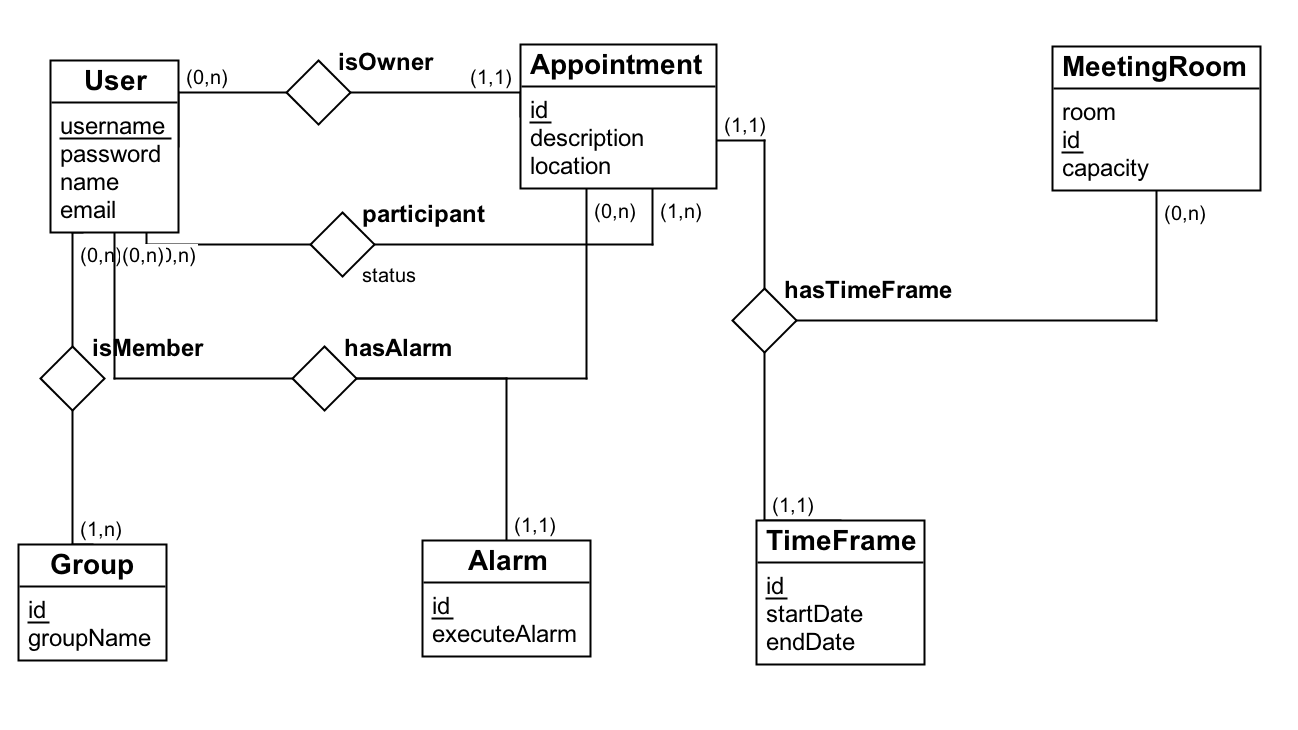
\includegraphics[width=8cm]{erdiagram.png}
        \caption{ER diagram}
    \label{class}
    \end{center}
\end{figure}

\subsection*{Krav 1}
Username and password is located in the User entity, the program checks if the username is correct against the database.

\subsection*{Krav 2}
A user creates an appointment by writing a description and selecting a start and end date, the database automaticly assigns an id to the appointment and the program creates a TimeFrame in the database and connects it to the appointment.

\subsection*{Krav 3}
The appointment creator adds users to a meeting, the program tells the database to add relation between a user and the appointment.The database also records the status of a participant in the participant relation. If a group is invited the program will iterate over the members and add them.

\subsection*{Krav 4}
The appointment creator changes some information about the event, and the program changes it in the database.

\subsection*{Krav 5}
The appointment creator deletes the appointment and it is removed from database.

\subsection*{Krav 6}
User sends a capacity request and a timeframe for a meeting room and the server fetches all the rooms that meets the criteria on capacity from the database and finds all available meeting rooms in the given timeframe and returns it to the user.

\subsection*{Krav 7}
A user wants to see his or her week overview and the program fetches the participant relations for this user and creates a overview for him or her.

\subsection*{Krav 8}
A user checks the participants for an appointment and the program fetches the status fields for that appointment from the database and returns it to the user.

\subsection*{Krav 9}
A user declines an invitation to join an appointment, the program alert all users with this message, and changes the status field in the database for this user and this appointment.

\subsection*{Krav 12}
This will be much like Krav 7, where the program fetches all the participant relations which has a status field where you can find information about the status of a participant.

\subsection*{Krav 13}
This will be much like Krav 7, but instead of fetching information for only one user, you get for several.

\subsection*{Krav 14}
A user adds an alarm to his appointment, the program creates a new alarm in the database with a date to execute.




\end{document}
